\chapter{System architecture}
\label{chapter:generalframework}
\smtrat is a \Cpp library consisting of a collection of
SMT compliant implementations of methods for solving non-linear real
and integer arithmetic \supportedLogics formulas, we refer to as modules. These modules can be 
combined to (1) a theory solver in order to extend the supported logics of an
existing SMT solver by \supportedLogics (see Figure~\ref{fig:frameworkb}) or (2) an SMT 
solver for \supportedLogics (see Figure~\ref{fig:frameworka}). The latter is 
especially intended to be a testing environment for the development 
of SMT compliant implementations of further methods tackling \supportedLogics. Here,
the developer only needs to implement the given interfaces of an \smtrat 
module and does not need to care about parsing input files, transforming
formulas to conjunctive normal form or embedding a SAT solver in order
to solve the Boolean skeleton of the given formula. Instead, \smtrat
provides this and more features, such as lemma exchange, which will be explained in following (taken from the system architecture description of our SAT'15 submission).

\begin{figure}[ht]
\caption{A snapshot of an \smtrat composition being an SMT solver for NRA.}
\begin{center}
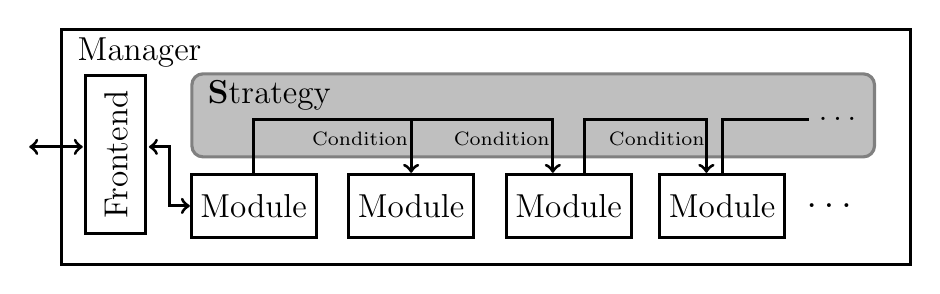
\begin{tikzpicture}[every node/.style={rectangle}, text centered, bend angle=15, line width=.4mm]
	\node[draw, minimum height=57pt, text width=15pt] (manager) at (-6.3, .2) {};
	\node[rotate=90] (managerText) at (-6.3, .2) {\large Frontend};
	\node[draw, minimum height=85pt, text width=300pt] (manager) at (-1.6, 0.3) {};
	\node[] (managerText) at (-6, 1.5) {\large Manager};
	\node[fill=lightgray,draw=gray, rounded corners, minimum height=30pt, text width=240pt] (strategy) at (-1,.7) {};
	\node[] (strategyText) at (-4.35, .95) {\large\textbf Strategy};
	\draw[<->] (-5.36,-.45) -- (-5.62,-.45) -- (-5.62,.3) -- (-5.88,.3);
	\draw[<->] (-6.72,.3) -- (-7.4,.3);
	\draw[->] (-4.55,-.03) -- (-4.55,.65) -- (-.75,.65) -- (-.75,-.03);
	\node[] (strategyText) at (-1.4, .4) {\scriptsize Condition};
	\draw[->] (-2.55,.65) -- (-2.55,-.03);
	\node[] (strategyText) at (-3.2, .4) {\scriptsize Condition};
	\draw[->] (-.35,-.03) -- (-0.35,.65) -- (1.2,.65) -- (1.2,-.03);
	\node[] (strategyText) at (.57, .4) {\scriptsize Condition};
	\draw (1.4,-.03) -- (1.4,.65) -- (2.5,.65);
	\node[] (dotsa) at (2.9,.65) {\large \ldots};
	\node[draw, minimum height=23pt] (moduleAText) at (-4.55, -.45) {\large Module};
	\node[draw, minimum height=23pt] (moduleBText) at (-2.55, -.45) {\large Module};
	\node[draw, minimum height=23pt] (moduleCText) at (-.55, -.45) {\large Module};
	\node[draw, minimum height=23pt] (moduleDText) at (1.4, -.45) {\large Module};
	\node[] (dotsc) at (2.8, -.45) {\Large \ldots};
\end{tikzpicture}%

\end{center}
\label{fig:frameworka}
\end{figure}

\begin{figure}[ht]
\caption{A snapshot of an \smtrat composition being a theory solver embedded in an SMT solver.}
\begin{center}
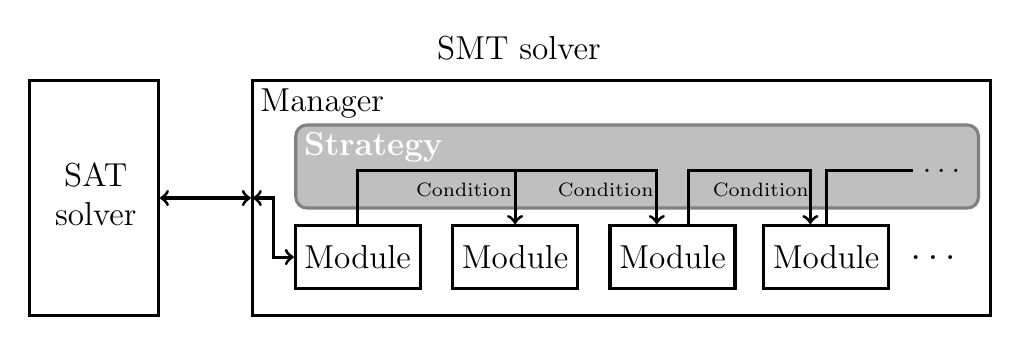
\begin{tikzpicture}[every node/.style={rectangle}, text centered, bend angle=15, scale=1, line width=.4mm]
	\node[] (smtsolver) at (-2.5, 2.2) {\large SMT solver};
	\node[draw, minimum height=85pt, text width=40pt] (satsolver) at (-7.9, 0.3) {\large\begin{tabular}{c}SAT \\ solver\end{tabular}};
	\node[draw, minimum height=85pt, text width=260pt] (manager) at (-1.2, 0.3) {};
	\node[] (managerText) at (-5, 1.5) {\large Manager};
	\node[fill=lightgray,draw=gray, rounded corners, minimum height=30pt, text width=240pt] (strategy) at (-1,.7) {};
	\node[] (strategyText) at (-4.35, .95) {\large\bf \color{white} Strategy};
	\draw[<->] (-5.36,-.45) -- (-5.62,-.45) -- (-5.62,.3) -- (-5.88,.3);
	\draw[->] (-4.55,-.03) -- (-4.55,.65) -- (-.75,.65) -- (-.75,-.03);
	\node[] (strategyText) at (-1.4, .4) {\scriptsize Condition};
	\draw[->] (-2.55,.65) -- (-2.55,-.03);
	\node[] (strategyText) at (-3.2, .4) {\scriptsize Condition};
	\draw[->] (-.35,-.03) -- (-0.35,.65) -- (1.2,.65) -- (1.2,-.03);
	\node[] (strategyText) at (.57, .4) {\scriptsize Condition};
	\draw (1.4,-.03) -- (1.4,.65) -- (2.5,.65);
	\node[] (dotsa) at (2.9,.65) {\large \ldots};
	\node[draw, minimum height=23pt] (moduleAText) at (-4.55, -.45) {\large Module};
	\node[draw, minimum height=23pt] (moduleBText) at (-2.55, -.45) {\large Module};
	\node[draw, minimum height=23pt] (moduleCText) at (-.55, -.45) {\large Module};
	\node[draw, minimum height=23pt] (moduleDText) at (1.4, -.45) {\large Module};
	\node[] (dotsc) at (2.8, -.45) {\Large \ldots};
	\path[<->] (satsolver.0) edge[] node[left] {} (manager.180);
\end{tikzpicture}

\end{center}
\label{fig:frameworkb}
\end{figure}

Based on \carl's data structures and basic functions, a rich set of SMT compliant implementations of \supportedLogics procedures is provided by \smtrat. Each procedure is encapsulated in a \emph{module}, which fixes a common interface, and they can then be composed to a solver according to a user defined \emph{strategy}. A \emph{manager} maintains their allocation to \emph{solving tasks} according to the strategy and provides the API, including the parsing of an \smtlibfile.

\section{Modules}
A module $m$ holds a set of formulas, called its \emph{set of received formulas} and denoted by $\Crcv(m)$. The main function of a module is \texttt{check(bool full)}, which either decides whether $\Crcv(m)$ is satisfiable or not, returning \SAT or \UNSAT, respectively, or returns \UNKNOWN. A set of formulas is semantically defined by their conjunction. If the function's argument \texttt{full} is set to \false, the underlying procedure of $m$ is allowed to omit hard obstacles during solving at the cost of returning \UNKNOWN in more cases. We can manipulate $\Crcv(m)$ by adding (removing) formulas $\varphi$ to (from) it with \texttt{add($\varphi$)} (\texttt{remove($\varphi$)}). Usually, $\Crcv(m)$ is only slightly changed between two consecutive \texttt{check} calls, hence, the solver's performance can be significantly improved if a module works incrementally and supports backtracking. In case $m$ determines the unsatisfiability of $\Crcv(m)$, it has to compute at least one preferably small \emph{infeasible subset} $\Cinf(m)\subseteq \Crcv(m)$. Moreover, a module can specify \emph{lemmas}, which are valid formulas. They encapsulate information which can be extracted from a module's internal state and propagated among other modules. Furthermore, a module itself can ask other modules for the satisfiability of its \emph{set of passed formulas} denoted by $\Cpass(m)$, if it invokes the procedure \texttt{runBackends(bool full)} (controlled by the manager). It thereby delegates work to modules that	 may be more suitable for the problem at hand. 

\section{Strategy}
\label{sec::strategy}
\smtrat allows a user to decide how to compose the modules. For this purpose we provide a graphical user interface, where the user can create a \emph{strategy} specifying this composition. A strategy is a directed tree $T:=(V, E)$ with a set $V$ of modules as nodes and $E\subseteq V\times \Omega\times\Sigma\times V$, with $\Omega$ being the set of \emph{conditions} and $\Sigma$ being the set of \emph{priority values}. A condition is an arbitrary Boolean combination of formula properties, such as propositions about the Boolean structure of the formula, e.g., whether it is in conjunctive normal form (CNF), about the constraints, \eg whether it contains equations, or about the polynomials, e.g., whether they are linear. Furthermore, each edge carries a unique priority value from $\Sigma=\{1,\ \ldots,\ |E|\}$.

\section{Manager}
\label{sec::manager}
The \emph{manager} holds the strategy and the SMT solver's input formula $C_{input}$. Initially, the manager calls the method \texttt{check} of the module $m_r$ given by the root of the strategy with $\Crcv(m_r) = C_{input}$. Whenever a module $m\in V$ calls \texttt{runBackends}% for its passed formula $\Cpass(m)$
, the manager adds a \emph{solving task} $(\sigma,\ m,\ m')$ to its priority queue $Q$ of solving tasks (ordered by the priority value), if there exists an edge $(m,\ \omega,\ \sigma,\ m')\in E$  in the strategy such that $\omega$ holds for $\Cpass(m)$. If a processor $p$ on the machine where \smtrat is executed on is available, the first solving task of $Q$ is assigned to $p$ and popped from $Q$. The manager thereby starts the method \texttt{check} of $m'$ with $\Crcv(m') = \Cpass(m)$ and passes the result (including infeasible subsets and lemmas) back to $m$. The module $m$ can now benefit in its solving and reasoning process from this shared information. Note that a strategy-based composition of modules works incrementally and supports backtracking not just within one module but as a whole. This is realized by a mapping in each module $m$ of its passed formulas $\varphi\in\Cpass(m)$ to sets $R_1,\ldots,\ R_n \subseteq \Crcv(m)$ such that each $R_i$ forms a reason why $m$ included $\varphi$ in $\Cpass(m)$ to ask for its satisfiability. In order to exploit the incrementality of the modules, all parallel executed backends terminate in a consistent state (instead of just being killed), if one of them finds an answer.
  
\section{Procedures implemented as modules}
\label{sec:implemented_modules}
The heart of an SMT solver usually forms a SAT solver. In \smtrat, the module \satModule abstracts $\Crcv(\satModule)$ to propositional logic and uses the efficient SAT solver \minisat~\cite{minisat} to find a Boolean assignment of the abstraction. It invokes \texttt{runBackends} where $\Cpass(\satModule)$ contains the constraints abstracted by the assigned Boolean variables in a less-lazy fashion~\cite{sebastiani2007lazy}. The module \simplexModule implements the Simplex method equipped with branch-and-bound and cutting-plane procedures as presented in \cite{DM06}. We apply it on the linear constraints of any conjunction of \supportedLogics constraints. For a conjunction of nonlinear constraints \smtrat provides the modules \gbModule, \vsModule and \cadModule, implementing GB~\cite{JLCA_CAI13}, VS~\cite{Article_Corzilius_FCT2011} and CAD~\cite{Article_Loup_TubeCAD} procedures, respectively. Moreover, the module \icpModule uses ICP similar as presented in~\cite{GGIGSC10}, lifting splitting decisions and contraction lemmas to a preceding \satModule and harnessing other modules for nonlinear conjunctions of constraints as backends. The exact procedure is going to be published. The module \cnfModule invokes \texttt{runBackends} on $\Cpass(\cnfModule)$ being the CNF of $\Crcv(\cnfModule)$, and the module \ppModule performs some preprocessing based on factorizations and sum-of-square decompositions of polynomials.

\section{Infeasible subsets and lemmas}
\label{sec::infsubset_lemmas}
Infeasible subsets and lemmas, which contain only formulas from 
$\Cpass(\SATM)$, prune the Boolean search space and hence the number of theory calls. 
Smaller infeasible subsets are usually more advantageous, because they make larger cuts 
in the search space. Lemmas containing new constraints we call
\emph{inventive lemmas} (\emph{non-inventive} otherwise). They might enlarge the 
Boolean search space, but they can reduce the complexity of later theory calls.
When using inventive lemmas, it is important to ensure that the set possible
constraints introduced in such lemmas is finite for a given module and a given 
input formula. Otherwise, the termination of this procedure can not be guaranteed.

